
%(BEGIN_QUESTION)
% Copyright 2006, Tony R. Kuphaldt, released under the Creative Commons Attribution License (v 1.0)
% This means you may do almost anything with this work of mine, so long as you give me proper credit

Studer denne glidespindelventilen med aktuator, og avgjør om den er luft-til-åpne eller luft-til-lukke. Avgjør også hva ventilen gjør (lukker, åpner eller blir stående) dersom trykkluftforsyningen faller bort:

$$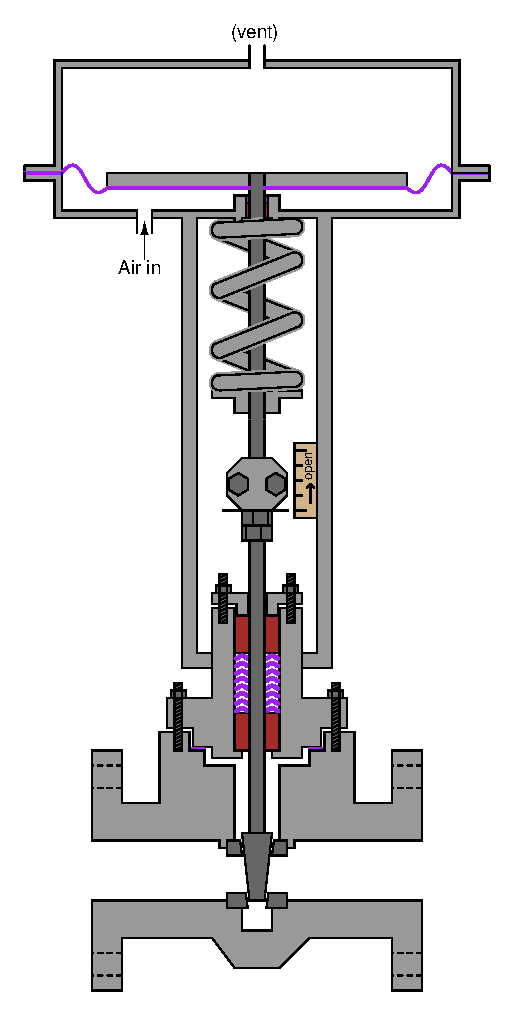
\includegraphics[height=10.5cm]{i00784x01.eps}$$

\vskip 20pt \vbox{\hrule \hbox{\strut \vrule{} {\bf Forslag til sokratisk diskusjon} \vrule} \hrule}

\begin{itemize}
\item{} Er dette en {\it direkte}- eller {\it revers}-virkende aktuator?
\item{} Er dette et {\it direkte}- eller {\it revers}-virkende ventilhus?
\item{} Jobber fjæren i {\it strekk}- eller {\it trykk}-modus?
\end{itemize}

\underbar{file i00784}
%(END_QUESTION)





%(BEGIN_ANSWER)


%(END_ANSWER)





%(BEGIN_NOTES)

Dette er en {\it luft-til-åpne}-ventilsammenstilling, siden ventilmekanismen er direktevirkende (spindel opp for å åpne) og aktuatoren er reversvirkende (spindel går opp ved økende lufttrykk). Den vil feile {\it lukket} ved bortfall av luftforsyning.

\vskip 10pt

Som instruktør bør du være bevisst at ordene «åpen» og «lukket» kan skape forvirring hos studenter med mye erfaring fra elektriske brytere. For ventiler betyr «åpen» fri gjennomstrømning. For brytere betyr «åpen» brutt krets. Tilsvarende får «lukket» motsatt betydning for reguleringsventiler kontra elektriske brytere.

\vfil \eject

\noindent
{\bf Forberedelsesquiz:}

Feilmodusen til en reguleringsventil bestemmes av:

\begin{itemize}
\item{} Typen pakkemateriale brukt for å tette prosessfluid
\vskip 5pt
\item{} Type ventilsats (f.eks. port-guided, cage-guided)
\vskip 5pt
\item{} Type aktuatorfluid (f.eks. luft kontra hydraulikkolje)
\vskip 5pt
\item{} Retningen ventilen installeres i prosessrøret
\vskip 5pt
\item{} Bench-set-verdiene til aktuatoren (f.eks. 3-15 PSI, 6-20 PSI)
\vskip 5pt
\item{} Retningen den interne fjæren skyver ventilsatsen
\end{itemize}


%INDEX% Sluttkontrollelementer, ventil: luft-til-åpne versus luft-til-lukke
%INDEX% Sluttkontrollelementer, ventil: feilsikker

%(END_NOTES)


